\subsection{Tests}

Para verificar el correcto funcionamiento del algoritmo decidimos tomar varias configuraciones iniciales que nos parecían importante tomar en cuenta:

\begin{figure}[H]
 \centering
  \subfloat[]{
   \label{sinSol}
    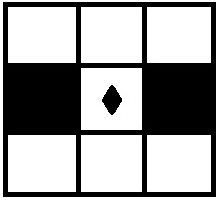
\includegraphics[width=0.1\textwidth]{ej3/imgs/ejSinSolucion.png}}
  \subfloat[]{
   \label{f:peorCaso}
    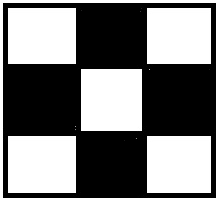
\includegraphics[width=0.1\textwidth]{ej3/imgs/ajedrezDibujo.png}}
  \subfloat[]{
   \label{f:grilla1}
    
\includegraphics[width=0.1\textwidth]{ej3/imgs/1x3.png}}
  \subfloat[]{
   \label{f:grilla2}
    
\includegraphics[scale=0.32]{ej3/imgs/3x1.png}}
  \subfloat[]{
   \label{f:cuatri}
    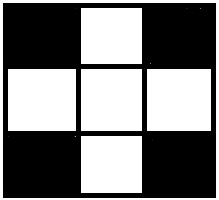
\includegraphics[width=0.1\textwidth]{ej3/imgs/cuatridireccional.png}}
 \caption{Varias configuraciones}
 \label{f:configs}
\end{figure}

Nos interesó analizar estas configuraciones porque:

\begin{itemize}
	\item[(a)] no tiene solución.
	\item[(b)] es un caso que presenta muchas paredes.
	\item[(c) y (d)] son grillas no cuadradas.
	\item[(e)] es un caso en donde con un sensor se pueden cubrir todos los casilleros.
\end{itemize}

Los resultados obtenidos fueron:

\begin{figure}[H]
 \centering
  \subfloat[]{
   \label{f:sinSol}
    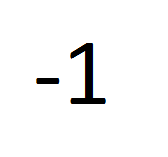
\includegraphics[width=0.1\textwidth]{ej3/imgs/1.png}}
  \subfloat[]{
   \label{f:peorCaso}
    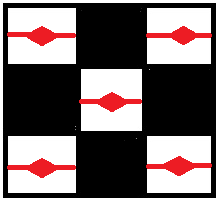
\includegraphics[width=0.1\textwidth]{ej3/imgs/ajedrezSol.png}}
  \subfloat[]{
   \label{f:grilla1}
    
\includegraphics[width=0.1\textwidth]{ej3/imgs/1x3Sol.png}}
  \subfloat[]{
   \label{f:grilla2}
    
\includegraphics[scale=0.32]{ej3/imgs/3x1Sol.png}}
  \subfloat[]{
   \label{f:cuatri}
    
\includegraphics[width=0.1\textwidth]{ej3/imgs/cuatridireccionalSol.png}}
 \caption{Soluciones}
 \label{f:configs}
\end{figure}

En todos los casos la solción devuelta fue la óptima a excepción del primero en donde no había solución.
